\documentclass[letterpaper, 12pt]{report}

% administrivia
\usepackage[utf8]{inputenc}
\usepackage[T1]{fontenc}
\usepackage[english]{babel}
\usepackage[nottoc, numbib]{tocbibind}
\usepackage{hyperref}

% alt dette for ett eksempel
\usepackage[footnotesize, bf, hang]{caption}
\usepackage{subcaption}
\usepackage{floatrow}
\usepackage{calc}
\floatsetup{ 
	heightadjust=object,
	valign=t
}

% layout
%\usepackage{fullpage}
\usepackage{mathpazo}
\usepackage{inconsolata}
\usepackage{hyperref}
\usepackage{enumitem}
\usepackage{setspace}
\onehalfspacing
\frenchspacing
\usepackage{listings}
\lstset{
	basicstyle=\ttfamily\footnotesize,%\scriptsize, 
	tabsize=2, 
	breaklines=true
}
\usepackage{wrapfig}
\usepackage{graphicx}

% citation
\usepackage[
	style=authoryear, 
	backend=biber, 
	dateabbrev=false
]{biblatex}
\addbibresource{references.bib}
\DefineBibliographyStrings{english}{%
	urlseen = {Retrieved},
}

\usepackage{lipsum}

% front matter
\title{\Huge \textbf{Measuring Productivity in the Software Engineering Industry}}
\author{
	Håkon S. Mork \\ 
	ORGB 423 --- Human Resources Management \\ 
	McGill University \\
	\\
	\emph{With the kind contribution of Solfrid Skilbrigt}
}
\date{\today}

\begin{document}
\maketitle
\tableofcontents

\chapter{Introduction}
\section{Objectives}
Lorem ipsum dolor sit amet, consectetur adipisicing elit, sed do eiusmod tempor incididunt ut labore et dolore magna aliqua. Ut enim ad minim veniam, quis nostrud exercitation ullamco laboris nisi ut aliquip ex ea commodo consequat. Duis aute irure dolor in reprehenderit in voluptate velit esse cillum dolore eu fugiat nulla pariatur. Excepteur sint occaecat cupidatat non proident, sunt in culpa qui officia deserunt mollit anim id est laborum.

\section{Company}
Steria is a multinational company founded in 1969 that specializes in information technology consulting, services and management. 
With headquarters in Paris and French administration, Steria is present in 16 countries and on three continents. 
The company boasts more than 20,000 employees and a 2011 annual revenue of €1.75 billion \parencite{steria:stats}.

\section{Human Resources Professional}
\begin{wrapfigure}{r}{0.3\textwidth}
	\centering
	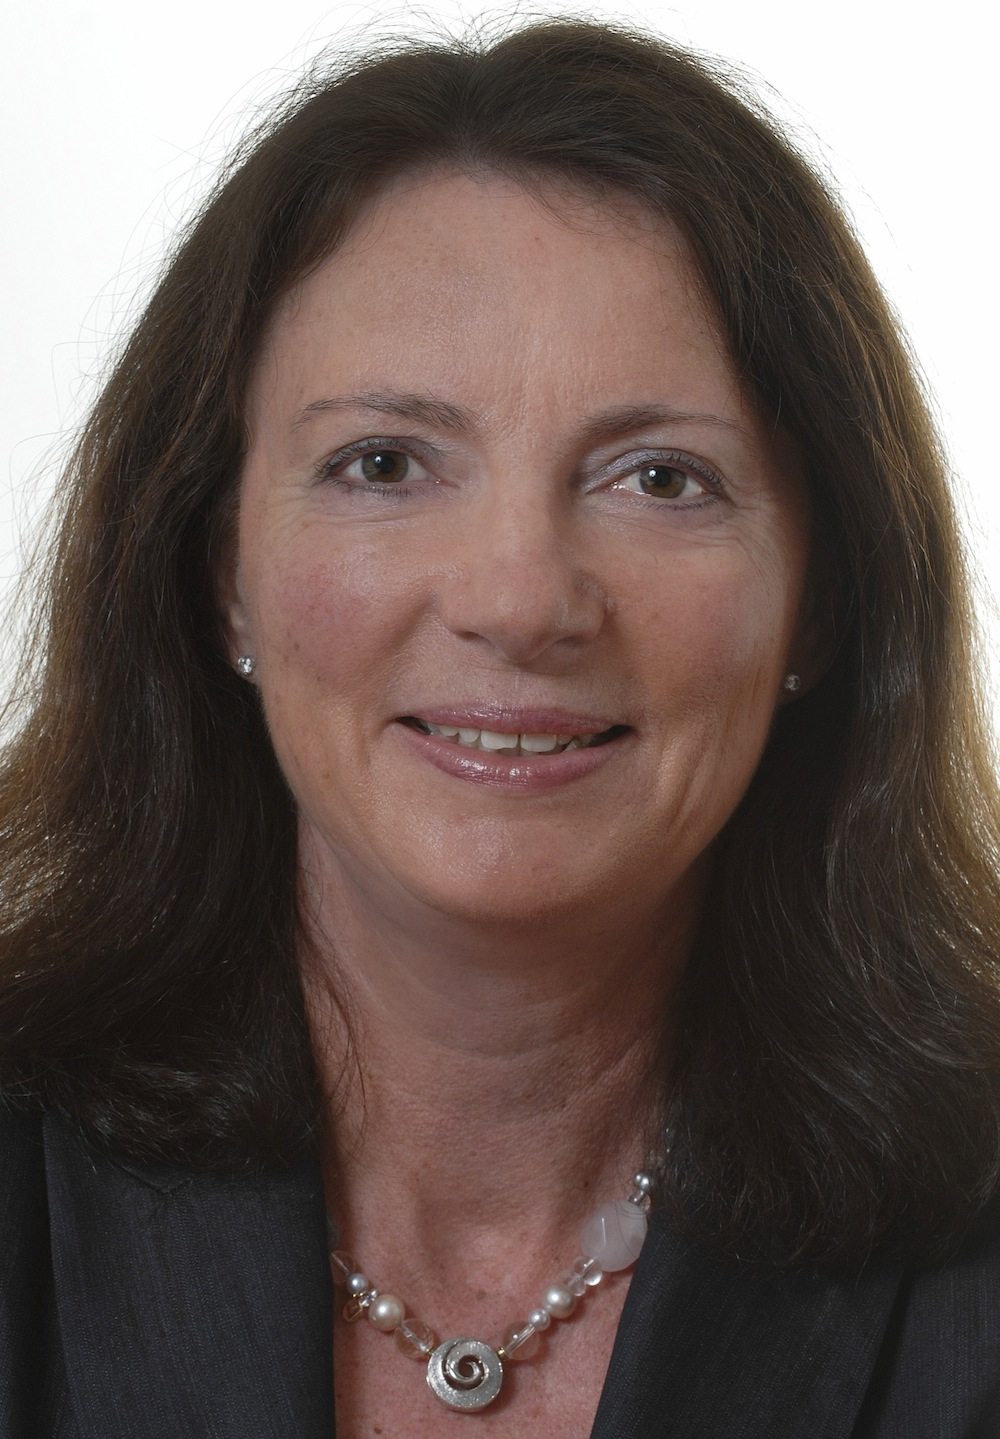
\includegraphics[width=\textwidth]{solfrid}
	\caption*{Solfrid Skilbrigt}
\end{wrapfigure}
Solfrid Skilbrigt, Human Resouces Director of the Norwegian and Scandinavian branch and Deputy CEO of Scandinavia, has kindly agreed to answer my questions about human resource management in her firm. 
A graduate of the University of Trondheim, she has long and varied experience in the fields of information technology, sales, and human resources.
Her accomplishments include leading the company's employer branding, recruitment, and management and organizational development programs, as well as playing a key part in Steria's advancement to being one of the world's leading IT consulting firms. 
Skilbrigt has also been in charge of Steria's global CSR efforts since 2008.


\section{Topic Area}
%cite \cite{goossens93} 
%citep \citep{goossens93}.

\chapter{Main Part}
\section{Basics of Software Engineering}

\section{Challenges of Measuring Productivity}
\subsection{The Nature of Software}
Indeed, \textcite{graham:succinctness} argues that terseness

\subsection{External Conditions}

\section{Discussion}

% language length example
% (fold)
\newsavebox{\pythonexample}
\begin{lrbox}{\pythonexample}
\begin{lstlisting}
n = int(input())
for i in range(1, n + 1):
	print i
\end{lstlisting}
\end{lrbox}

\newsavebox{\cexample}
\begin{lrbox}{\cexample}
\begin{lstlisting}
#include <stdio.h>
int main(int argc, char **argv) 
{
	int n;
	scanf("%d", &n);
	int i;
	for (i = 1; i < n + 1; i++) 
	{
		printf("%d\n", i);
	}
	return 0;
}
\end{lstlisting}
\end{lrbox}

\begin{figure}
\ffigbox{
	\begin{subfloatrow}
		\ffigbox[\FBwidth+1em]{\usebox{\cexample}}{\subcaption{Example in C}}
		\ffigbox[\FBwidth+1em]{\usebox{\pythonexample}}{\subcaption{Example in Python}}
	\end{subfloatrow}
}
{\caption{These two pieces of computer code, in two different programming languages, do exactly the same thing---yet one is four times longer than the other.}}
\end{figure}
% (end)

\section{Industry Practice}

\chapter{Conclusion}

\appendix

\chapter{Interview Questions}
\begin{enumerate}[leftmargin=*]
	\item What is your (full) name?
	\item How old are you?
	\item What is your Birthday?
	\item What starsign does that make it?
	\item What is your favourite colour?
	\item What is your lucky number?
	\item Do you have any pets?
	\item What shoe size are you?
	\item How many pairs of shoes do you own?
	\item If you were prime miniser or ruler of the world, what laws would you make?
	\item If you were a super hero, what powers would you have?
\end{enumerate}

\chapter{Letter of Thanks}
Thanks!

%\nocite{*}
% \bibliographystyle{apacite}
% \bibliography{references}
\phantomsection
\addcontentsline{toc}{chapter}{Bibliography}
\printbibliography

\end{document}
